%
% Optional reading
%

\begin{frame}[plain,c]
\begin{center}
{\Huge \bf Optional reading for Lecture \thislecture}
\end{center}
\end{frame}

% ------------------------------------------------------------------------------

%
% Worked example :
%

{
\problemslide

\begin{frame}{Worked example: Exploiting the superposition principle}

  \begin{blockexmplque}{Question}
    A nonconductive solid sphere has a uniform volume charge density $\rho$.\\
    \vspace{0.1cm}
    Let $\vec{r}$ be the vector from the centre of the sphere to a general point
    $P$ within the sphere. As you should be able to easily confirm,
    the electric field $\vec{E}$ at a point $\vec{r}$  within the sphere is
    given by $\vec{E}(\vec{r}) = \rho \vec{r}/(3\epsilon_0)$.\\
    \vspace{0.1cm}
    If a spherical cavity is hollowed out of the sphere, as shown below,
    using superposition concepts, show that the electric field at all points
    within the cavity is uniform and equal to
    $\vec{E}(\vec{r})=\rho \vec{a}/(3\epsilon_0)$
    where $\vec{a}$ is the position vector
    from the centre of the sphere to the centre of the cavity.\\
    \begin{center}
      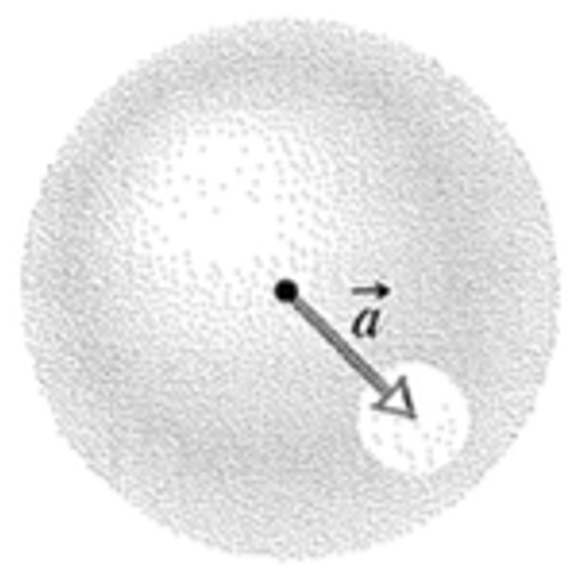
\includegraphics[width=0.20\textwidth]{./images/problems/lect02_spherical_charge_distribution_with_hole}
    \end{center}
  \end{blockexmplque}

\end{frame}

%
%
%

\begin{frame}{Worked example: Exploiting the superposition principle}

  The charge distribution in case of a uniformly charged solid sphere
  with a cavity is equivalent to that of
  a whole uniformly charged solid sphere of charge density $\rho$
  plus a smaller uniformly charged solid sphere
  of charge density -$\rho$ that fills the void.\\
  \vspace{0.2cm}

  \begin{columns}
    \begin{column}{0.38\textwidth}
      \begin{center}
        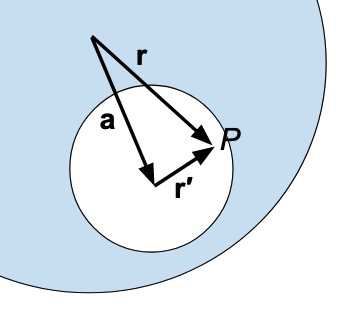
\includegraphics[width=0.95\textwidth]{./images/problems/lect02_sphere_with_cavity_distances_2}
      \end{center}
    \end{column}
    \begin{column}{0.62\textwidth}
      The field produced by each uniformly charged sphere is given.\\
      By superposition, the field at a point $P$ within the cavity
      (at distance $\vec{r}$ from the centre of the larger sphere)
      is given by
      \begin{equation*}
        \vec{E}(\vec{r}) =
        \frac{\rho \vec{r}}{3 \epsilon_0} +
        \frac{(-\rho) \vec{r}^\prime}{3 \epsilon_0} =
           \frac{\rho \vec{r}}{3 \epsilon_0} +
           \frac{(-\rho) (\vec{r} - \vec{a})}{3 \epsilon_0} \Rightarrow
      \end{equation*}
      \begin{equation*}
        \vec{E}(\vec{r}) =
           \frac{\rho \vec{a}}{3 \epsilon_0}
      \end{equation*}
    \end{column}
  \end{columns}

\end{frame}

} %\problemslide


% ------------------------------------------------------------------------------

%
% Worked example :
%

{
\problemslide

\begin{frame}{Worked example: Spherical shell with non-uniform density}

  \begin{blockexmplque}{Question}
    A spherical shell of inner radius $a$ and outer radius $b$ has volume charge
    density $\rho = kr^2$ ($a \le r \le b$), where $k$ is a constant and $r$ is
    the radial distance from the centre of the shell.\\
    Find the magnitude of the electric field $\vec{E}$
    produced by this charge distribution
    at radial distances i) $r<a$, ii) $a \le r < b$, and iii) $b \le r$.
  \end{blockexmplque}

  \vspace{0.2cm}

  Due to the obvious spherical symmetry, the electric field $\vec{E}$
  is a radial vector, and it is
  is going to be a function of only the radial distance $r$.\\

  \vspace{0.2cm}

  We have 3 distinct regions:
  i) $r<a$, ii) $a \le r < b$, and iii) $b \le r$.
  \vspace{0.2cm}

  For the calculation of $\vec{E}$ we will be applying Gauss's theorem:
  \begin{equation*}
    \int_{S} \vec{E} \cdot d\vec{S} =
      \frac{Q_{encl}}{\epsilon_0} =
        \frac{1}{\epsilon_0} \int_{\tau(S)} \rho d\tau
  \end{equation*}

\end{frame}

%
%
%

\begin{frame}{Worked example: Spherical shell with non-uniform density}

  For $r<a$, for {\em any possible} closed surface $S$
  that stays within that region of no charge, Gauss's theorem gives
  \begin{equation*}
    \int_{S} \vec{E} \cdot d\vec{S} = 0
  \end{equation*}
  Since this happens for all surfaces, it can not be the result of an
  accidental cancellation and it has to be that the integrand itself is 0.
  Therefore:
  \begin{equation}
    E (r<a) = 0
  \end{equation}

  \vspace{0.2cm}

  For $a \le r < b$, exploiting the spherical symmetry,
  we will be applying Gauss's theorem
  for a concentric spherical surface $S(r)$ of radius $r$.\\

  \vspace{0.2cm}

  Because both $\vec{E}$ and the surface vector $d\vec{S}$ are collinear,
  and the norm of $\vec{E}$ is constant, everywhere on $S(r)$,
  the flux calculation is simplified:
  \begin{equation*}
    \int_{S(r)} \vec{E} \cdot d\vec{S} =
    \int_{S(r)} E dS =
    E \int_{S(r)} dS =
    E 4\pi r^2
  \end{equation*}

\end{frame}

%
%
%

\begin{frame}{Worked example: Spherical shell with non-uniform density}

  The charge $Q_{enc}$, in the volume $\tau(S)$,
  enclosed by a spherical surface $S(r)$ of radius $r$
  is given by:
  \begin{equation*}
    Q_{enc} =
      \int_{\tau(S)} \rho d\tau =
      \int_{a}^{r} \Big( k u^2 \Big) 4\pi u^2 du =
      4\pi k \int_{a}^{r} u^4 du =
      \frac{4\pi k}{5} u^5 \Big\rvert_{a}^{r} \Rightarrow
  \end{equation*}
  \begin{equation*}
      Q_{enc} =
      \frac{4\pi k}{5} \Big(r^5 - a^5\Big)
  \end{equation*}

  Therefore, Gauss's law can be expressed as:
  \begin{equation*}
    E \cancel{4\pi} r^2 =
     \frac{\cancel{4\pi} k}{5 \epsilon_0} \Big(r^5 - a^5\Big)
  \end{equation*}

  This yields:
  \begin{equation*}
    E (a \le r < b)= \frac{k}{5 \epsilon_0} \Big(r^3 - \frac{a^5}{r^2}\Big)
  \end{equation*}

\end{frame}

%
%
%

\begin{frame}{Worked example: Spherical shell with non-uniform density}

  For $b \le r$, one can apply a similar analysis. In this case,
  $Q_{enc}$ is no longer a function of $r$
  since all spherical surfaces $S(r)$ include all charge.
  From the previous expression for $Q_{enc}$,
  setting $r$ equal to $b$, we have:
  \begin{equation*}
    Q_{enc} =
      \frac{4\pi k}{5} \Big(b^5 - a^5\Big)
  \end{equation*}

  Gauss's law can be expressed as:
  \begin{equation*}
    E \cancel{4\pi} r^2 =
     \frac{\cancel{4\pi} k}{5 \epsilon_0} \Big(b^5 - a^5\Big)
  \end{equation*}

  This yields:
  \begin{equation*}
    E (b \le r)= \frac{k}{5 \epsilon_0} \Big(\frac{b^5 - a^5}{r^2}\Big)
  \end{equation*}

  Summarizing, we found that:
  \begin{equation*}
    \displaystyle
    E =
      \begin{cases}
        0 & \text{ for } r < a\\
        \frac{k}{5 \epsilon_0} \Big(r^3 - \frac{a^5}{r^2}\Big) & \text{ for } a \le r < b\\
        \frac{k}{5 \epsilon_0} \Big(\frac{b^5 - a^5}{r^2}\Big) & \text{ for } b \le r
      \end{cases}
  \end{equation*}

\end{frame}

} %\problemslide


% ------------------------------------------------------------------------------

{
\programmingslide

%
%
%

\begin{frame}{PHYS201 scientific programming task for Lecture \thislecture}

{\small

If you did the previous task, you already have a program to calculate the
electric field (in 2-D) for an arbitrary distribution of discrete charges.\\
\vspace{0.2cm}

Generalize your previous program:
\begin{itemize}
{
  \item Move from a 2-D to a {\bf 3-D calculation}.
  \item Add an option to {\bf specify a continuous distribution of charge}
        (i.e. work with a user-defined charge density function $\rho(\vec{r})$)
}
\end{itemize}

\vspace{0.2cm}
What you will be doing, is to perform the following numerical integration:
\begin{equation*}
   \vec{E}(\vec{r}) = \frac{1}{4\pi\epsilon_0} \int_{\tau}
      d\tau^{\prime} \frac{\rho({\pvec{r}'})}{|\vec{r}-\pvec{r}'|^{3}} (\vec{r}-\pvec{r}')
\end{equation*}

\vspace{0.3cm}

Can you test Gauss' law numerically?

}
\end{frame}

%
%
%

\begin{frame}{PHYS201 scientific programming task for Lecture \thislecture}

{\small

As an example, use the following charge density in spherical coordinates:
\begin{equation*}
   \rho =
     \begin{cases}
       \frac{\rho_0}{(r/r_0)^2} e^{-r/r_0} cos^2\phi, & \text{if $r < 5 r_0$} \\
       & \\
       0, \text{otherwise}
     \end{cases}
\end{equation*}
where $\rho_0$ = 0.16 C/m$^{3}$ and r$_0$ = 10 cm.\\
%
% at r = 5 *r0, the charge contained is 6.24 * \rho_0 * ro^3
% 0.16 is 1/6.24
%

\vspace{0.2cm}
Calculate numerically the amount of charge Q enclosed in a sphere of radius r, as a function or r:\\
\begin{equation*}
  Q(r) = \int_{0}^{r} \int_{4\pi} d\tau \rho(\vec{r^\prime})
\end{equation*}

\vspace{0.2cm}
Confirm that your distribution plateaus to a value of $Q_{tot}$ for
r $>5r_0$, as the sphere encloses all regions of non-zero charge density.
What is the value of $Q_{tot}$?\\

\vspace{0.2cm}
Calculate the electric flux through the surface of a sphere with radius r = 5$r_0$
and confirm that:
\begin{equation*}
  \epsilon_0 \oint \vec{E} \cdot d\vec{S} = Q_{tot}
\end{equation*}
}

\end{frame}

} % programming
